\subsubsection{Asynchron UART (Debug Interface)}
\label{sec:CubeMXUart}

Auf dem DSP Board sind die beiden Pins \texttt{PA9 (Rx)} und \texttt{PA10 (Rx)} auf Testpoints geführt. 
Über die UART Schnittstelle \texttt{USART1} kann ein Serieller Adapter angeschlossen werden.
Die Abbildung \ref{pic:CubeMX_Uart} zeigt die Standardeinstellungen mit einer Baudrate von $115200 \si{Bd}$. Interrupts oder DMA werden nicht verwendet.

\begin{figure}[H]
	\centering
	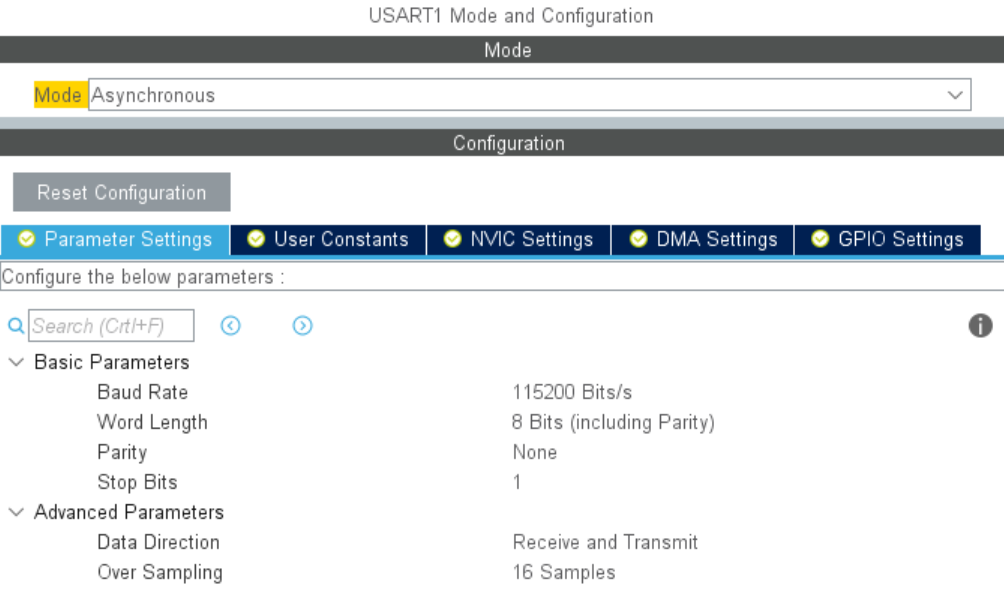
\includegraphics[width=1.0\linewidth]{CubeMX_Uart}
	\caption{Parameter Einstellungen der USART1 Schnittstelle}
	\label{pic:CubeMX_Uart}
\end{figure}


